\documentclass{beamer}
\usetheme{CambridgeUS}

%----macros begin-----------------------------------------------------------------------------------
\usepackage{graphicx}
\usepackage{color}
\usepackage{xcolor}
\usepackage{amsfonts}
\usepackage{amsmath}
%\usepackage{amsthm}
%\usepackage[utf8]{inputenc}
\usepackage{framed}
\usepackage{wasysym}

\newcommand{\columnsbegin}{\begin{columns}}
\newcommand{\columnsend}{\end{columns}}

%\renewenvironment{Shaded}{\pause\begin{snugshade}}{\end{snugshade}}
\def\twocolumns#1#2{\begin{columns}
\begin{column}{0.5\linewidth}#1\end{column}
\begin{column}{0.5\linewidth}#2\end{column}
\end{columns}}
\def\mytwocolumns#1#2#3#4{\begin{columns}
\begin{column}{#1\linewidth}#2\end{column}
\begin{column}{#3\linewidth}#4\end{column}
\end{columns}}
\def\mythreecolumns#1#2#3#4#5#6{\begin{columns}
\begin{column}{#1\linewidth}#2\end{column}
\begin{column}{#3\linewidth}#4\end{column}
\begin{column}{#5\linewidth}#6\end{column}
\end{columns}}
\def\threecolumns#1#2#3{\begin{columns}
\begin{column}{0.33\linewidth}#1\end{column}
\begin{column}{0.33\linewidth}#2\end{column}
\begin{column}{0.33\linewidth}#3\end{column}
\end{columns}}
\def\fourcolumns#1#2#3#4{\begin{columns}%
\begin{column}{0.25\linewidth}#1\end{column}%
\begin{column}{0.25\linewidth}#2\end{column}%
\begin{column}{0.25\linewidth}#3\end{column}%
\begin{column}{0.25\linewidth}#4\end{column}%
\end{columns}}

\def\textbf#1{\alert{#1}}
\def\emph#1{{\color{cyan}#1}}
\def\conv{\mbox{\textrm{conv}\,}}
\def\aff{\mbox{\textrm{aff}\,}}
\def\E{\mathbb{E}}
\def\R{\mathbb{R}}
\def\Z{\mathbb{Z}}
\def\N{\mathbb{N}}
\def\P{\mathbb{P}}
\def\v#1{{\bf #1}}
\def\p#1{{\bf #1}}
\def\T#1{{\bf #1}}
\def\vet#1{{\left(\begin{array}{cccccccccccccccccccc}#1\end{array}\right)}}
\def\mat#1{{\left(\begin{array}{cccccccccccccccccccccccccccc}#1\end{array}\right)}}

\def\lin{\mbox{\rm lin}\,}
\def\aff{\mbox{\rm aff}\,}
\def\pos{\mbox{\rm pos}\,}
\def\cone{\mbox{\rm cone}\,}
\def\conv{\mbox{\rm conv}\,}
\newcommand{\homog}[0]{\mbox{\rm homog}\,}
\newcommand{\relint}[0]{\mbox{\rm relint}\,}

\newtheorem{assignment}{Assignment}
\newtheorem{exercise}{Exercise}
\newtheorem{question}{Question}
\newtheorem{remark}{Remark}
%----macros end-----------------------------------------------------------------------------------

\newcommand\myenum[1]{% 
  \begin{pgfpicture}{-1ex}{-0.65ex}{1ex}{1ex} 
    \usebeamercolor[fg]{item projected} 
    {\pgftransformscale{1.75}\pgftext{\normalsize\pgfuseshading{bigsphere}}} 
    {\pgftransformshift{\pgfpoint{0pt}{0.5pt}} 
      \pgftext{\usebeamerfont*{item projected}#1}} 
  \end{pgfpicture}% 
} 

\definecolor{whitesmoke}{HTML}{F5F5F5}

%
%\usepackage{listings}
%\lstdefinestyle{bash-style}{
%  captionpos=b,
%  belowcaptionskip=1\baselineskip,
%  breaklines=true,
%  tabsize=2,
%  frame=tb,
%  aboveskip=3mm,
%  belowskip=3mm,
%  xleftmargin=\parindent,
%  language=bash,
%  showstringspaces=false,
%  % basicstyle=\tiny, %\footnotesize\ttfamily,
%  basicstyle={\fontsize{8pt}{8pt}\ttfamily},
%  keywordstyle=\color{black},
%  commentstyle=\color{green!40!black},
%  stringstyle=\color{brown},
%  identifierstyle=\color{black},
%  backgroundcolor=\color{whitesmoke}
%}
%\lstdefinestyle{python-style}{
%  captionpos=b,
%  belowcaptionskip=1\baselineskip,
%  breaklines=true,
%  tabsize=2,
%  frame=tb,
%  aboveskip=3mm,
%  belowskip=3mm,
%  xleftmargin=\parindent,
%  language=Python,
%  showstringspaces=false,
%  % basicstyle=\tiny, %\footnotesize\ttfamily,
%  basicstyle={\fontsize{8pt}{8pt}\ttfamily},
%  keywordstyle=\color{blue},
%  commentstyle=\color{green!40!black},
%  stringstyle=\color{brown},
%  identifierstyle=\color{blue},
%  backgroundcolor=\color{whitesmoke}
%}


% Default fixed font does not support bold face
\DeclareFixedFont{\ttb}{T1}{txtt}{bx}{n}{12} % for bold
\DeclareFixedFont{\ttm}{T1}{txtt}{m}{n}{12}  % for normal

% Custom colors
\usepackage{color}
\definecolor{deepblue}{rgb}{0,0,0.5}
\definecolor{deepred}{rgb}{0.6,0,0}
\definecolor{deepgreen}{rgb}{0,0.5,0}
\definecolor{whitesmoke}{HTML}{F5F5F5}

\usepackage{listings}

% Python style for highlighting
\newcommand\pythonstyle{\lstset{
language=Python,
basicstyle=\ttm,
otherkeywords={self},             % Add keywords here
keywordstyle=\ttb\color{orange},
emph={MyClass,__init__},          % Custom highlighting
emphstyle=\ttb\color{deepred},    % Custom highlighting style
stringstyle=\color{deepgreen},
frame=tb,                         % Any extra options here
showstringspaces=false,           % 
  captionpos=b,
  belowcaptionskip=1\baselineskip,
  breaklines=true,
  tabsize=2,
  frame=tb,
  aboveskip=3mm,
  belowskip=3mm,
  xleftmargin=\parindent,
  language=Python,
  showstringspaces=false,
  basicstyle=\footnotesize\ttfamily,
  basicstyle={\fontsize{8pt}{8pt}\ttfamily},
  % keywordstyle=\color{blue},
  commentstyle=\color{deepgreen}\slshape,
  stringstyle=\color{brown},
  identifierstyle=\color{blue},
% language=python,
% basicstyle=\ttfamily\scriptsize\setstretch{1},
% stringstyle=\color{red},
% showstringspaces=false,
% alsoletter={1234567890},
% otherkeywords={\ , \}, \{},
% keywordstyle=\color{blue},
emph={access,and,break,class,continue,def,del,elif ,else,%
except,exec,finally,for,from,global,if,import,in,i s,%
lambda,not,or,pass,print,raise,return,try,while},
emphstyle=\color{black}\bfseries,
emph={[2]True, False, None, self},
emphstyle=[2]\color{green},
emph={[3]from, import, as},
emphstyle=[3]\color{red},
upquote=true,
morecomment=[s]{"""}{"""},
%commentstyle=\color{gray}\slshape,
emph={[4]1, 2, 3, 4, 5, 6, 7, 8, 9, 0},
% emphstyle=[4]\color{blue},
%literate=*{:}{{\textcolor{blue}:}}{1}%
%{=}{{\textcolor{blue}=}}{1}%
%{-}{{\textcolor{blue}-}}{1}%
%{+}{{\textcolor{blue}+}}{1}%
%{*}{{\textcolor{blue}*}}{1}%
%{!}{{\textcolor{blue}!}}{1}%
%{(}{{\textcolor{blue}(}}{1}%
%{)}{{\textcolor{blue})}}{1}%
%{[}{{\textcolor{blue}[}}{1}%
%{]}{{\textcolor{blue}]}}{1}%
%{<}{{\textcolor{blue}<}}{1}%
%{>}{{\textcolor{blue}>}}{1},%  
  backgroundcolor=\color{whitesmoke}
}}


% Python environment
\lstnewenvironment{python}[1][]
{
\pythonstyle
\lstset{#1}
}
{}

% Python for external files
\newcommand\pythonexternal[2][]{{
\pythonstyle
\lstinputlisting[#1]{#2}}}

% Python for inline
\newcommand\pythoninline[1]{{\pythonstyle\lstinline!#1!}}



% \usepackage{beamerthemesplit} // Activate for custom appearance

\usepackage{listings}

% Default fixed font does not support bold faced
\DeclareFixedFont{\ttb}{T1}{txtt}{bx}{n}{12} % for bold
\DeclareFixedFont{\ttm}{T1}{txtt}{m}{n}{12}  % for normal

% Custom colors
\usepackage{color}
\definecolor{deepblue}{rgb}{0,0,0.5}
\definecolor{deepred}{rgb}{0.6,0,0}
\definecolor{deepgreen}{rgb}{0,0.5,0}

\definecolor{whitesmoke}{HTML}{F5F5F5}


\usepackage{listings}


\title{Geometric \& Graphics Programming Lab: Lecture 7}
\author{Alberto Paoluzzi}
\date{\today}

\nonstopmode



\begin{document}

\frame{\titlepage}

\section[Outline]{}
\frame{\tableofcontents}


\section{2D Affine Transformations -- (1)}
%- SLIDE ----------------------------------------------------------------------
\begin{frame}\frametitle{Introduction}\small

\vfill

\begin{itemize}
\vfill\item 
\emph{Affine transformations} are used to map a figure or model into another of different size, position or orientation; 

\vfill\item 
they reduce to an invertible linear transformationby using \href{http://robotics.stanford.edu/~birch/projective/node4.html}{\emph{homogeneous coordinates}}

\vfill\item 
fixed a reference system, they are represented by squared invertible matrices, said \emph{transformation matrices}

\vfill\item 
we study the structure and properties of \emph{``elementary'' transformations} of 2D plane and 3D space.
\end{itemize}

\vfill
\end{frame}
%- SLIDE ----------------------------------------------------------------------
%- SLIDE ----------------------------------------------------------------------
\begin{frame}\frametitle{Assumptions}\small

\vfill
\begin{itemize}
\vfill\item vectors and points are represented as \emph{column vectors}

\vfill\item\vspace{-1mm} transformations are given by \emph{left products} by a matrix: $\v{v}^*=\T{M}\v{v}$

\vfill\item\vspace{-1mm} the \emph{reference frame} is assumed \emph{left-handed }
\end{itemize}

\vfill

\begin{center}
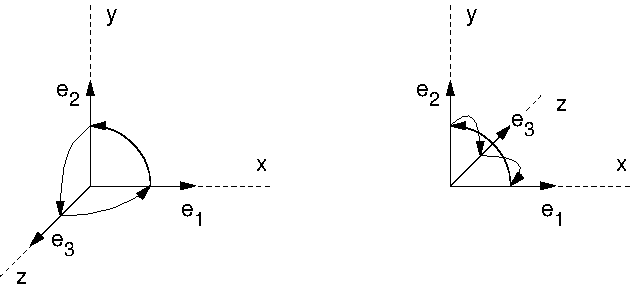
\includegraphics[height=40mm]{images/riferimenti1}
\end{center}

\alert{positive rotations}: (a)~right-handed frame
(b)~left-handed frame

\end{frame}
%- SLIDE ----------------------------------------------------------------------
\begin{frame}\frametitle{Homogeneous coordinates}\small

\vfill

define a \emph{bijective mapping} between the set of \emph{points} of Cartesian plane and the set of \emph{lines through the origin} $\p{o}$ of 3D space

\vfill
\begin{center}
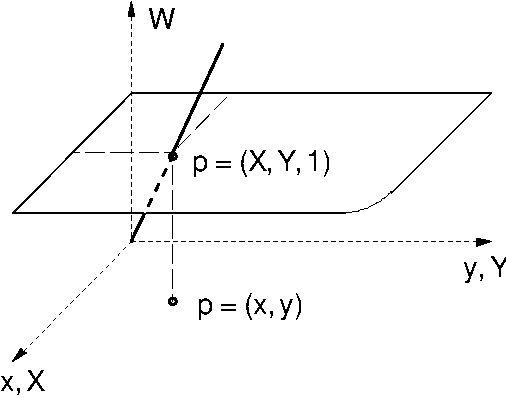
\includegraphics[width=0.5\linewidth]{images/omogenee}
\end{center}
\vfill

{Homogeneous coordinates of 2D plane}

\end{frame}
%- SLIDE ----------------------------------------------------------------------
\begin{frame}\frametitle{Homogeneous coordinates} \small

\vfill
in such  $\E^2\rightarrow \E^3$ mapping, every point $(x, y)^T\in{\E}^2$ is represented as the set of points 
\[
\{(X, Y, W)^T\in{\E}^3 \  | \ x=X/W,\ y = Y/W,\ W\not= 0\}
\]


\vfill

to transform the homogeneous point  $\p{p}' = (X, Y, W)$ into the Cartesian point $\p{p} = (x, y)$ two divisions by the homogeneous coordinate $W$ are needed.  

\vfill

to avoid this computation we use the \emph{homogeneous normalized representation} $(X, Y, 1)^T$, such that
\[
x = X, \qquad y = Y
\]

\vfill

the point $(x, y)^T$ of plane is represented by a vector $\lambda (x, y, 1)^T$, with $\lambda\in\R$ e $\lambda \not=0$.
\end{frame}

\subsection{Translation}

%- SLIDE ----------------------------------------------------------------------
\begin{frame}\frametitle{Translation}\small

\vfill

A \emph{translation} of 2D plane is a function $\T{T}: \E^{2}\rightarrow \E^{2}$, where a fixed vector $\v{t} = (m, n)^T$ is summed to each point $\p{p} = (x, y)^T$, so that

\[
\p{p}^* = \T{T}(\p{p}) = \p{p} + \v{t} =
\vet{x \\ y} + \vet{m \\ n} =
\vet{x+m \\ y+n} .
\]

\vfill
\centering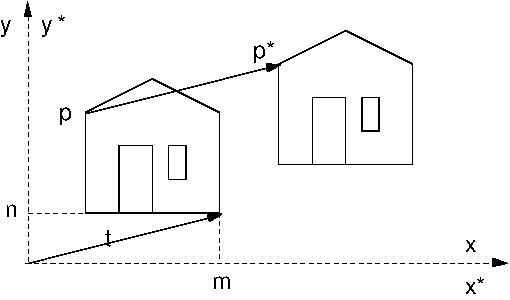
\includegraphics[height=40mm]{images/traslazione}
\vfill
\end{frame}
%- SLIDE ----------------------------------------------------------------------
\begin{frame}\frametitle{Traslation}\small

\vfill
A movement of origin implies that the translation is not a linear transformation. Therefore, it cannot be represented in coordinates by a matrix

\vfill

\emph{the translation is linear when using homogeneous coordinates}. In fact, the translation that maps the $\p{p}$ point to
\[
\p{p}^*=\p{p}+\v{t},
\]

with $\v{t}=(m,n)^T$, becomes, in homogeneous coordinates:

\[
\p{p}^* = \T{T}\ \p{p} =
\mat{
1 &  0 &  m\\
0 &  1 &  n\\
0 &  0 &  1
}
\vet{ x \\  y \\  1 }
=
\vet{ x+m \\ y+n \\ 1}
\]

\vfill
\end{frame}
%- SLIDE ----------------------------------------------------------------------
\begin{frame}[fragile]
\frametitle{Translation}\small

 \emph{Higher-order functions} need a double application over (a) integer specificators and (b) real parameters, in order to generate the \emph{transformation tensor} 

\vfill

\centering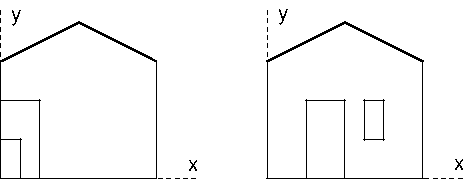
\includegraphics[width=0.5\linewidth]{images/smallhouse1}

\vfill

write the code to do the above example

\end{frame}

\subsection{Scaling}

%- SLIDE ----------------------------------------------------------------------
\begin{frame}\frametitle{Scaling}
\framesubtitle{definition}

\vfill

A \emph{scaling}  $\T{S}$ is a transformation tensor represented by a \emph{diagonal matrix} with positive coefficients, so that:

\[
\p{p}^* = \T{S}\ \p{p} =
\mat{
a & 0 \\
0 & b
}\vet{x \\ y}
= \vet{ax \\ by},
\qquad
a,b >0
\]

\vfill

\begin{itemize}
\vfill\item 
if $a,b>1$, then $\T{S}$ is a \emph{dilatation} tensor
\vfill\item 
if $a=b=1$, then $\T{S}$ is the \emph{identity} tensor
\vfill\item 
if $a,b<1$, then $\T{S}$ is a \emph{compression} tensor
\end{itemize}

\vfill
\end{frame}
%- SLIDE ----------------------------------------------------------------------
\begin{frame}\frametitle{Scaling}
\framesubtitle{elementary scalings}\small

\vfill

\begin{minipage}[c]{6cm}
\[
\p{p}^* = \T{S}_x\ \p{p} =
\mat{
a & 0 \\
0 & 1
}
\vet{x \\ y}
= \vet{ax \\ y}
\]\end{minipage}\hfill~



\vfill
\begin{center}
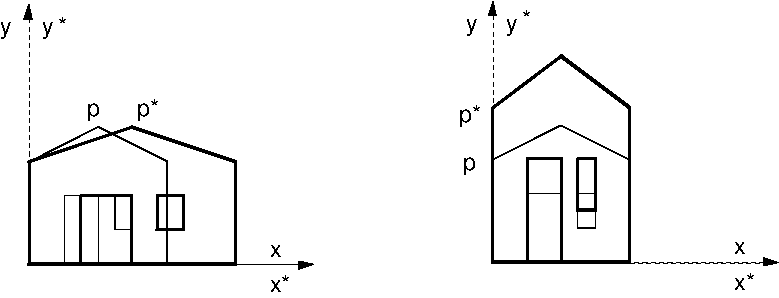
\includegraphics[height=30mm]{images/scala1}
\end{center}
\vfill

~\hfill\begin{minipage}[c]{6cm}
\[
\p{p}^* = \T{S}_y\ \p{p} =
\mat{
1 & 0 \\
0 & b
}
\vet{x \\ y}
= \vet{x \\ by}
\]\end{minipage}

\end{frame}
%- SLIDE ----------------------------------------------------------------------
\begin{frame}\frametitle{Scaling}
\framesubtitle{homogeneous coordinates}

\vfill

the homogeneous normalized coordinate matrix $\T{S}'\in \R^3_{3}$ of a 2D scaling tensor may be easily derived  from the non-homogeneous matrix
 $\T{S}\in \R^2_{2}$, by adding a unit row and column:

\vfill

\[
\p{p}^* =
\T{S}'\p{p} =
\mat{
\T{S} & \T{0}\\
\T{0} &  1
}
\vet{x \\ y \\ 1}
=
\mat{
a & 0 & {0}\\
0 & b & {0}\\
0 &{0} &  1
}
\vet{x \\ y \\ 1}
=
\vet{ax \\ by \\ 1} .
\]

\vfill
\end{frame}
%- SLIDE ----------------------------------------------------------------------
\begin{frame}\frametitle{Scaling}
\framesubtitle{uniform scaling}\small

\vfill

When $a=b$ the scaling is said {\emph{uniform}} or \emph{homothetic} transformation

\vfill
\begin{enumerate}
    \vfill\item with $a=b=0.5$ the length of all segments is halved
    \vfill\item\vspace{-2mm} the image $\p{p}^{*}$ of each $\p{p}$ goes on the line through $\p{p}$ and the origin
    \vfill\item\vspace{-2mm} the transformed figure is also \emph{closer} to the origin
\end{enumerate}

\vfill

\begin{center}
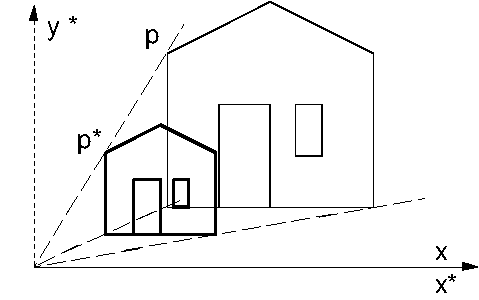
\includegraphics[height=33mm]{images/scala2}
\end{center}

\vfill
action of a  tensor of uniform scaling

\end{frame}
 %---------------------------------------------------------------------
\subsection{Reflection}
%- SLIDE ----------------------------------------------------------------------
\begin{frame}\frametitle{Reflection}
\framesubtitle{definition}

\vfill

Linear transformation defined by a matrix that differs from the identity since one of diagonal coefficients is  $-1$

\vfill

Two elementary reflections $\T{M}_{x}$ e $\T{M}_{y}$ may be defined in the plane $\E^{2}$

\[
\T{M}_{x}=\mat{-1 & 0 \\ 0 & 1}, \qquad
\T{M}_{y}=\mat{1 & 0 \\ 0 & -1}
\]

\vfill

The action of a reflection tensor inverts the sign of one of coordinates of points

\end{frame}
%- SLIDE ----------------------------------------------------------------------
\begin{frame}\frametitle{Reflection}
\framesubtitle{homogeneous representation}\small

\vfill
As usual, the normalized homogeneous representation of such transformations is obtained by adding a unit row and column to their matrices

\[
\T{M}'_{x}=\mat{\T{M}_{x} & \v{0} \\ \v{0} & 1}, \qquad
\T{M}'_{y}=\mat{\T{M}_{y} & \v{0} \\ \v{0} & 1}
\]


\vfill

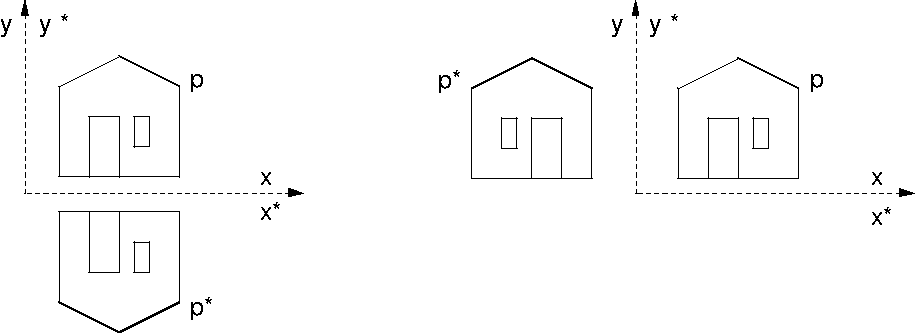
\includegraphics[width=\linewidth]{images/ribaltam}

\end{frame}
%- SLIDE ----------------------------------------------------------------------
\begin{frame}[fragile]
\frametitle{Reflection}
\framesubtitle{example}\small

Let us continue the house example by adding \emph{simmetry} to the scene
\vfill

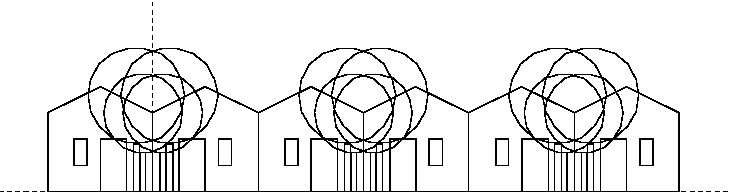
\includegraphics[width=\linewidth]{images/mirror}

\vfill


\end{frame}
%- SLIDE ----------------------------------------------------------------------
\section{2D Affine transformations -- (2)}
%---------------------------------------------------------------------- SLIDE -

\subsection{Rotation}

%- SLIDE ----------------------------------------------------------------------
\begin{frame}\frametitle{Elementary rotation of plane}\small

\vfill

An \emph{elementary rotation} of 2D plane is a linear function that maps every point $\p{p}\in \E^{2}$ to the second extreme $\p{p}^{*}= \T{R}(\p{p})$ of a circle arc with first extreme in $\p{p}$,  center in the origin and constant angle $\alpha$

\vfill

The matrix of a rotation tensor is easily computed by considering the images of basis vectors $(\v{e}_i)$

\vfill

\[
\mat{
\v{e}_1^* & \v{e}_2^* }
=
\T{R}\ \mat{
\v{e}_1 & \v{e}_2  }.
\]
\vfill

where $\T{R}$ is the unknown rotation matrix 
\end{frame}
%- SLIDE ----------------------------------------------------------------------
\begin{frame}\frametitle{Elementary rotation of plane}

\vfill

more explicitly:

\[
\mat{
\cos\alpha & -\sin\alpha \\
\sin\alpha & \cos\alpha }
=
\T{R}\ \mat{
1 & 0 \\
0 & 1  },
\]

\vfill
\centering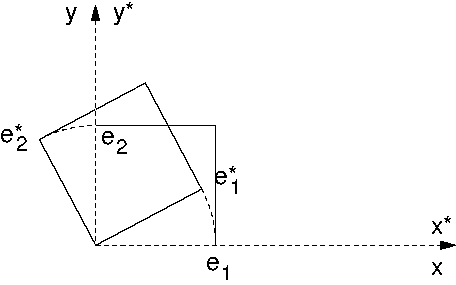
\includegraphics[height=35mm]{images/rot2D}
\vfill
\end{frame}
%- SLIDE ----------------------------------------------------------------------
\begin{frame}\frametitle{Elementary rotation of plane}
\framesubtitle{in homogeneous coordinates}

\vfill
The normalized homogeneous matrix $\T{R}' \in \lin \R^3$ of a plane rotation is obtained from the non-homogeneous matrix $\T{R}\in \lin \R^2$

\vfill

\[
\p{p}^* =
\T{R}'\p{p} =
\mat{
\T{R} & \T{0}\\
\T{0} &  1
}
\vet{x \\ y \\ 1}
=
\vet{x\ \cos\alpha+y\ \sin\alpha \\ -x\ \sin\alpha + y\ \cos\alpha \\ 1} 
\]
\vfill

in the usual way, by adding a unit row and column ...
 
\vfill
\end{frame}


%- SLIDE ----------------------------------------------------------------------
\begin{frame}[fragile]
\frametitle{Examples}
\framesubtitle{Elementary transformations in \texttt{pyplasm}}

\begin{python}
from larlib import *

filename = "test/svg/inters/house.svg"
lines = svg2lines(filename)
lines

VIEW(STRUCT(AA(POLYLINE)(lines)))
AA(POLYLINE)(lines)
house = STRUCT(AA(POLYLINE)(lines))
house

VIEW(STRUCT([house, T([1,2])([2,0.5])(house)]))
VIEW(STRUCT([house, S([1,2])([2,2])(house)]))
VIEW(STRUCT([house, S(1)(2)(house)]))
VIEW(STRUCT([house, S(1)(-1)(house)]))
VIEW(STRUCT([house, R([1,2])(PI/6)(house)]))
\end{python}

\end{frame}
%- SLIDE ----------------------------------------------------------------------
\subsection{Shearing}
%- SLIDE ----------------------------------------------------------------------
\begin{frame}\frametitle{Shearing}
\framesubtitle{elementary}

\vfill

The plane is seen as a \emph{bundle of lines} parallel to a coordinate axis

\vfill

A 2D \emph{elementary shearing} is a tensor which maps the points of a line in other points of the same line, in a way such that:

\vfill

\begin{enumerate}
    \vfill\item all points of a line translate by the same vector
    \vfill\item only the coordinate axis parallel to the line bundle remains fixed
    \vfill\item the translation of each line is proportional to its distance to the fixed line

\end{enumerate}
\vfill
\end{frame}
%- SLIDE ----------------------------------------------------------------------
\begin{frame}\frametitle{Shearing} \small

\vfill
An elementary shearing tensor \emph{does not change} one coordinate, whereas the other changes linearly with the value of the fixed coordinate

\[
\p{p}^* = \T{H}_x\ \p{p} = \mat{ 1 & 0\\
a & 1} \vet{ x \\ y} = \vet{ x \\ y + ax } ,
\]\vspace{-2mm}
\[
\p{p}^* = \T{H}_y\ \p{p} = \mat{ 1 & b\\
0 & 1 } \vet{ x \\ y } = \vet{ x + by \\ y } .
\]

\vfill
\centering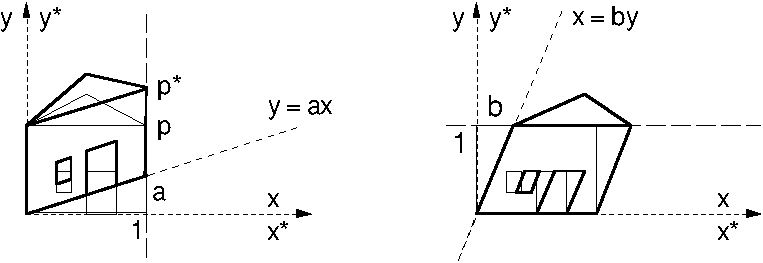
\includegraphics[width=0.8\linewidth]{images/deform}

Action of $\T{H}_{x}$, normal to the $x$ axis, and $\T{H}_{y}$, normal to the $y$ axis
\end{frame}
%- SLIDE ----------------------------------------------------------------------
\begin{frame}[fragile]
\frametitle{Shearing}
\framesubtitle{example}

\vfill

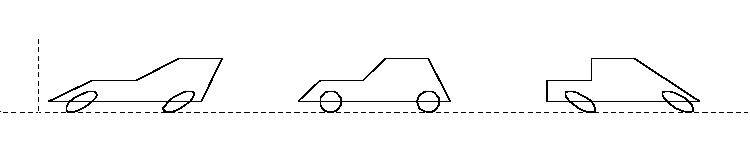
\includegraphics[width=\linewidth]{images/storyboard}


\end{frame}
%- SLIDE ----------------------------------------------------------------------
\begin{frame}[fragile]
\frametitle{Shearing}
\framesubtitle{example}

Three  \emph{keyframes} of the \emph{storyboard} of 3D animation entitled: ``My wife's car''

\vfill

\centering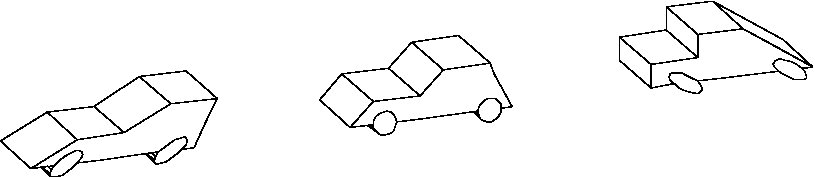
\includegraphics[width=\linewidth]{images/story3D}
\vfill


\end{frame}

\subsection{General transformations}

%- SLIDE ----------------------------------------------------------------------
\begin{frame}\frametitle{Arbitrary linear transformation}

\vfill

Let consider the action of a general $\T{Q}$  tensor on the unit square built on the basis of the Cartesian frame $(\p{o},
\v{e}_{i})$, with

\[
\T{Q} = \mat{a & c\\
             b & d}.
\]

arbitrary, but \emph{invertible matrix}

\vfill

such arbitrary linear transformation:

\begin{enumerate}
\vfill\item\vspace{-2mm} does not move the origin;
\vfill\item\vspace{-2mm} maps parallel lines to parallel lines;
\vfill\item\vspace{-2mm} does'nt conserve, in general, the size of areas.
\end{enumerate}

\end{frame}
%- SLIDE ----------------------------------------------------------------------
\begin{frame}\frametitle{General transformation}
\framesubtitle{action of a general tensor on the unit standard square}\small

\begin{center}
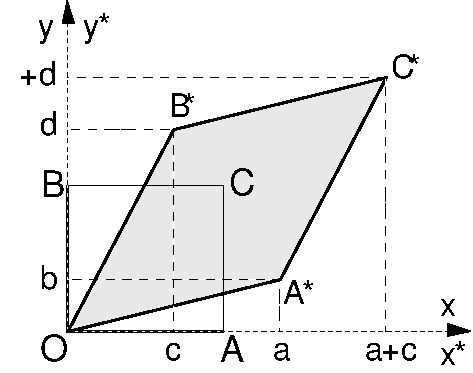
\includegraphics[height=30mm]{images/qualunque}
\end{center}

\[
\mat{
\p{o}^* & \p{a}^* & \p{b}^* & \p{c}^* }
=
\T{Q}\mat{
\p{o} & \p{a} & \p{b} & \p{c} },
\]

or, by using the corresponding  coordinates:
\[
\mat{
0 & a & c & a+c\\
0 & b & d & b+d}
=
\mat{
a & c\\
b & d
}
\mat{
0 & 1 & 0 & 1\\
0 & 0 & 1 & 1}.
\]

\end{frame}
%- SLIDE ----------------------------------------------------------------------
\begin{frame}\frametitle{Transformation with fixed point}
\framesubtitle{different from the origin}

\vfill

Every invertible linear transformation $\T{Q}$ has the origin $\p{o}$ of the Cartesian frame as its unique \emph{fixed point}, i.e. $\T{Q}(\p{o}) = \p{o}$

\vfill

To have a \emph{fixed point $\p{q}$ different from origin} we must compose three transformations, such that:

\vfill

\begin{enumerate}
\vfill\item map $\p{q}$ to the origin \p{o};
\vfill\item\vspace{-1mm} apply the required transformation;
\vfill\item\vspace{-1mm} map back \p{o} to $\p{q}$.
\end{enumerate}

\vfill
\end{frame}
%- SLIDE ----------------------------------------------------------------------
\begin{frame}\frametitle{Transformation with fixed point}
\framesubtitle{scaling}

\vfill
Let consider a \emph{scaling tensor} with fixed point $\p{q} =
(m,n)^{T} \not= \p{o}$:
\[
\T{S}_{\p{q}}(m, n, a, b) = \T{T}_{xy}(m, n)\circ \T{S}_{xy}(a,
b)\circ \T{T}_{xy}(-m, -n) .
\]

\vfill

\centering
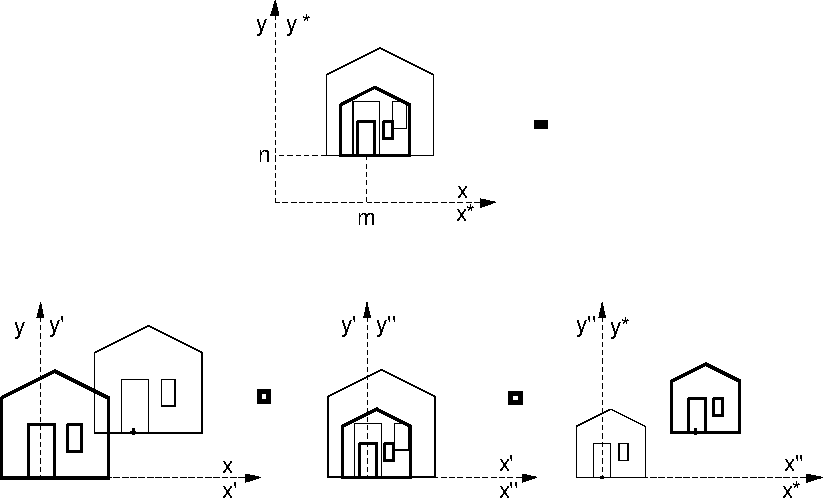
\includegraphics[width=0.8\linewidth]{images/scala3}
\vfill
scaling with fixed point as product of transformations
\end{frame}
%- SLIDE ----------------------------------------------------------------------
\begin{frame}\frametitle{Transformation with fixed point}
\framesubtitle{rotation}


\vfill
Let consider a \emph{rotation tensor} with fixed point $\p{q} =
(m,n)^{T} \not= \p{o}$:
\[
\T{R}_{\p{q}}(m, n, \alpha)
=\T{T}_{xy}(m, n)\circ \T{R}_{xy}(\alpha)\circ \T{T}_{xy}(-m, -n) .
\]

\vfill

\begin{center}
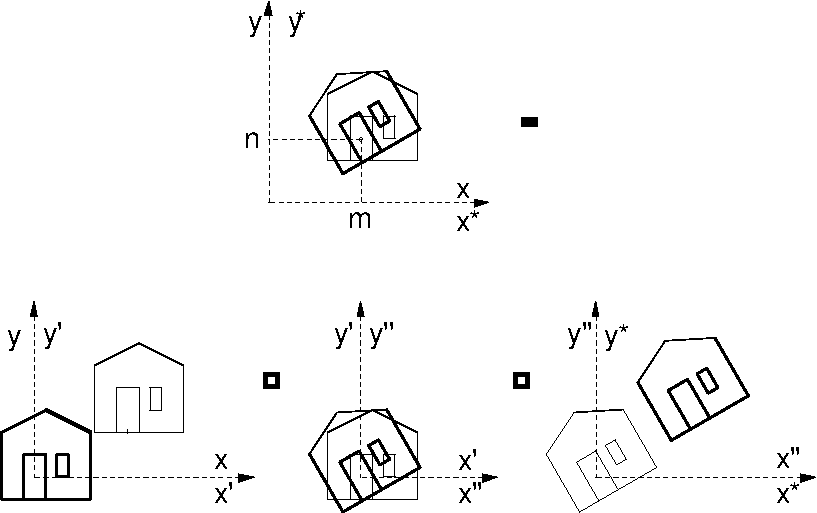
\includegraphics[width=0.7\linewidth]{images/rotfisso}
\end{center}

\vfill
rotation with fixed point as product of transformations

\end{frame}
%- SLIDE ----------------------------------------------------------------------
\begin{frame}[fragile]
\frametitle{2D Affine transformations}
\framesubtitle{example}

\centering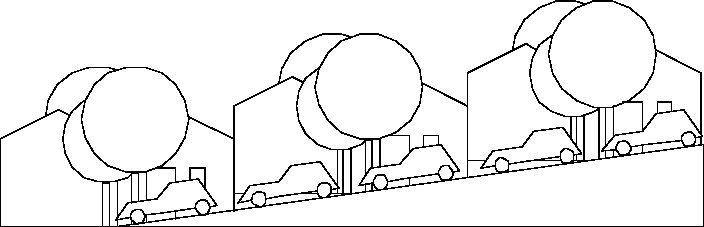
\includegraphics[width=0.8\linewidth]{images/InclinedTriple}

\vfill

\begin{remark}[Assignment]
Convert the example on pages 230-231 (chapter 6) of book \href{http://onlinelibrary.wiley.com/book/10.1002/0470013885}{\color{cyan} GP4CAD} from classic PLaSM (FL style) to \alert{pyplasm} \end{remark}

\end{frame}

\subsection{Representation of tensors}

%- SLIDE ----------------------------------------------------------------------
\begin{frame}[fragile]
\frametitle{Representation of tensors}

\vfill


Tensors are represented in PLaSM by applying the predefined function {\tt MAT}  to the tensor matrix (list of lists of coordinates)

\[
\mbox{\tt MAT} : \R^{3}_{3} \rightarrow \lin \R^{3}
\]

\vfill

Tensors, defined as linear endomorphisms of a vector space, have first-grade citizenship in PLaSM, and can be composed to generate new tensors. For example:

\vfill

Tensors can be applied to polyhedral complexes of arbitrary dimensions $(d,n)$

\end{frame}
%---------------------------------------------------------------------- SLIDE -

%- SLIDE ----------------------------------------------------------------------
\begin{frame}[fragile]
\frametitle{Representation of tensors}
\framesubtitle{example}

\begin{python}
from pyplasm import *

wall = MKPOL([  [[0,0],[4,0],[4,4],[2,6],[0,4]],
				[[1,2,3,4,5]],None  ])
Q = MAT([[1,0,0],[0,1,0.5],[0,0,1]])

VIEW(Q(wall))
\end{python}

\vfill 

Remember that: 

\begin{itemize}
\item
we use homogeneous coordinates (2D matrices are $3\times 3$);
\item
in PlaSM the homogeneous coordinate is the first
\end{itemize}

\end{frame}
%---------------------------------------------------------------------- SLIDE -
\end{document}

